% !TEX encoding = UTF-8
% !TEX TS-program = pdflatex
% !TEX root = ../tesi.tex

%**************************************************************
\chapter{Structure design}
\label{cap:structure-design}
%**************************************************************

The attacker knows that it is not easy to be accepted by his victim and, for this reason, he wants to understand what choices he must take to create the best profile possible to be accepted without too much delay by the victim. Therefore, the parameters must be defined based on the victim, to be accepted with greater possibility.
\par \noindent Thanks to the study of some specific papers mentioned above and thinking about how much to deepen the search for the best profile, in this chapter will be define and explain the chosen parameters. Then, from the parameters, the consequent profiles configurations will be shown.

%**************************************************************
\section{Project guidelines and the chosen parameters}
The definition of the parameters was conditioned by the degree of depth that the project wants to achieve: clearly more parameters lead to a greater number of profile configurations, but the data collection must be more in-depth and on a large scale. Furthermore, Facebook does not check that the date of birth that a user enters at the time of registration is true (therefore that he is really the age he claims to be) but that it only checks if it is valid for its standards (if it is at least 13 years old and if it's not existent like February 30th). This means that a person could enter data that is valid for Facebook but not true in reality. Assuming that there is always a real person behind a profile, untrue data would lead to an invalid analysis. Therefore, the parameters chosen are parameters that when registering on Facebook, a person would be required to be honest.\par \noindent 
It should be underlined how the resulting configuration of the profiles can be considered as the starting point: in the future the study could be deepened, adding other parameters, but this can be done by taking this as the starting configuration.

\subsection{First parameter: gender}
Gender is almost the most relevant factor, so much that most of the time is the decisive one. If looking at the profile's name, the gender is not clear, an user can check the bio of this profile. In fact, in the bio, the correspondent label of the gender will specify because a person who wants to register on Facebook must declare it and could be ``woman'', ``man'' or ``custom option'' where a user can set its pronouns. \par \noindent 
By the way, many papers of those cited report that a friend request from a female user profile is accepted easier than a friend request from a man user profile, regardless of the gender of the profile that receives it (an example of paper that report this statement is <<\textit{To be friend or not: a model of friend request acceptance}>>\parencite{site:paper7}, discussed on page \pageref{cap:to-be-friend}).
\subsubsection*{Classes}
The parameter \texttt{gender} $ \in \{$\texttt{female, male}$\}$, where: 
\begin{itemize}
	\item \texttt{female/F}, if the victim's profile user declares to be a \textit{female};
	\item \texttt{male/M}, if the victim's profile user declares to be a \textit{male}.
\end{itemize}
\subsection{Second parameter: image profile}
\label{cap:alt-technology}
The profile picture is the first thing, along with the name, a user sees when they have a friend request. As reported in some above-mentioned papers, the profile image already serves to give an idea of the person who is asking for friendship, because it shows some details that do not need to be checked (such as gender or an indicative age range).
A profile with a hidden or fake image (eg. a landscape) is more mysterious in the eyes of a user who receives the friend request, beacuse the real person behind this profile is not clearly identifiable. Therefore, the main idea is to verify the presence of at least one person in the profile picture and classify the user profiles based on the outcome of this verification.\par \noindent 
Facebook uses a technology that allows recognizing the profile image's content (faces, objects, ...) \parencite{site:alt-text} , and automatically creating a description that will be enclosed in the \texttt{alt} tag. 
The presence of one or more people (and occasionally other details about the panorama and/or some objects present) is always specified within the \texttt{alt} tag. On the other hand, if the image is fictional (cartoons, drawings, etc.) or is an image without a person (eg. landscapes), the \texttt{alt} tag contains ``\texttt{No description of the photo available}``. This technology has been exploited to classify each victim's profile picture.
\subsubsection*{Classes}
The parameter \texttt{real\_img} $ \in \{$\texttt{true,false}$\}$, where: 
\begin{itemize}
	\item \texttt{true}, if in \texttt{alt} tag reported the presence of one or more people;
	\item \texttt{false}, if in \texttt{alt} tag not reported the presence of one or more people;
\end{itemize}
\subsection{Third parameter: age} 
\label{cap:age-parameter}
Age is a very relevant factor. From the literature, it appears to be one of the first factors that a user who receives a friendship goes to check the profile from which the friend request started, if the age is not deducible from the image profile. 
The more similar age, the more likely it is that the friend request will be accepted. A person who wants to register on Facebook, must declare a real birth date (and must be at least 13 years old) and, once the profile has been created, can choose whether to make the date public or not. Some profiles publish only the month and day, other profiles only the year, others the complete date, others hide everything.\par \noindent To classify profile user's age, the date of birth that it reports will be taken, and the age will be calculated based on the current year, so as to be able to assign to this profile its membership class.
\subsubsection*{Classes}
Age is classified into 3 ranges, so the parameter \texttt{age\_range} $ \in \{2,3,4\}$, where: 
\begin{itemize}
	\item \texttt{2}, if the age victim's profile user is between 18 and 50 years;
	\item \texttt{3}, if the age victim's profile user is greater than 50 years;
	\item \texttt{4}, if the age victim's profile user is hidden;
\end{itemize}

\section{Parameters' configuration for creating profiles}
\label{cap:table-configuration}
To delineate the types of profiles (the same for both victims and attackers) it was necessary to define profile categories, which are nothing more than the combinations of all the various parameters.\par \noindent 
In this case study, the parameters that will be configured are:
\begin{enumerate}
	\item \texttt{gender} $ \in \{$\texttt{female, male}$\}$;
	\item \texttt{real\_img} $ \in \{$\texttt{true,false}$\}$;
	\item \texttt{age\_range} $ \in \{2,3,4\}$.
\end{enumerate}
Combining all various parameters with possible values, there are $12$ profiles and $12 \cdot 12 = 144$ possible attack combinations. All the various resulting configurations are now shown in Table \ref{table:configuration}:
\begin{table}[h!]
\begin{center}
	\begin{tabular}{ |c|c|c|c| } 
		\hline 
		\cellcolor[HTML]{b0d7ff} \texttt{gender} & 
		\cellcolor[HTML]{b0d7ff} \texttt{real\_img} & 
		\cellcolor[HTML]{b0d7ff} \texttt{age\_range} &
		\cellcolor[HTML]{b0d7ff} \textsc{label}	\\
		\hline 
		\texttt{female}	&	\texttt{true}	&	\textsc{2}	
		&	\cellcolor[HTML]{e6f2ff} \texttt{FT2}\\	 
		\hline
		\texttt{female}	&	\texttt{true}	&	\textsc{3}	
		&\cellcolor[HTML]{e6f2ff} \texttt{FT3}\\	 
		\hline
		\texttt{female}	&	\texttt{true}	&	\textsc{4}	
		& \cellcolor[HTML]{e6f2ff} \texttt{FT4}\\	 
		\hline
		\texttt{female}	&	\texttt{false}	&	\textsc{2}	
		& \cellcolor[HTML]{e6f2ff} \texttt{FF2}\\	 
		\hline
		\texttt{female}	&	\texttt{false}	&	\textsc{3}	
		& \cellcolor[HTML]{e6f2ff} \texttt{FF3}\\
		\hline
		\texttt{female}	&	\texttt{false}	&	\textsc{4}	
		& \cellcolor[HTML]{e6f2ff} \texttt{FF4}\\
		\hline 	
		\texttt{male}	&	\texttt{true}	&	\textsc{2}	
		& \cellcolor[HTML]{e6f2ff} \texttt{MT2}\\
		\hline
		\texttt{male}	&	\texttt{true}	&	\textsc{3}	
		& \cellcolor[HTML]{e6f2ff} \texttt{MT3}\\	 
		\hline
		\texttt{male}	&	\texttt{true}	&	\textsc{4}	
		& \cellcolor[HTML]{e6f2ff} \texttt{MT4}\\
		\hline
		\texttt{male}	&	\texttt{false}	&	\textsc{2}	
		& \cellcolor[HTML]{e6f2ff} \texttt{MF2}\\
		\hline
		\texttt{male}	&	\texttt{false}	&	\textsc{3}	
		& \cellcolor[HTML]{e6f2ff} \texttt{MF3}\\
		\hline
		\texttt{male}	&	\texttt{false}	&	\textsc{4}	
		& \cellcolor[HTML]{e6f2ff} \texttt{MF4}\\
		\hline 	 	 	 	 	
	\end{tabular}
	\caption{Profile configurations, identified by a label, based on the combinations of the parameters which are gender, age and profile picture.}
	\label{table:configuration}
\end{center}
\end{table}
\subsection*{The label}
As can be seen from the table above, each type of profile is classified with a \textit{label}. The label is the union of the actual value assumed by the parameters in that particular circumstance: the first character identifies the gender (``\texttt{F}'' in the case of ``\texttt{female}``, ``\texttt{M}'' in the case of ``\texttt{male}``), the second character indicates the value of the ``\texttt{real\_img}'' parameter (``\texttt{T}'' in case it is ``\texttt{true}``, ``\texttt{F}'' in case it is ``\texttt{false}``) and the last character is the numeric value that indicates the age range (it can be ``\texttt{2}``, ``\texttt{3}'' or ``\texttt{4}``). All \textit{victim profiles} are classified with these labels. In fact, each collected \textit{victim profile} is labeled into one of these $12$ categories.\par \noindent However, as regards the \textit{attackers} profiles, they will be created starting from these configurations and in an automated way with the help of the tool called \texttt{create-profile.py} (details in the Chapter \ref{cap:tool-create}). Furthermore, if attackers and victims have the same label it could be brought to create confusion in the second phase of the organization of the attack combinations. For this reason, the attackers' profiles are identified with an identifying code ``\texttt{PF-}\textit{n}'' where \textit{n} is an increasing identification number assigned when the profile is created. 

\section{Development planning}
Development takes place in 4 consecutive phases:
\begin{enumerate}
	\item  create the 12 attacker profiles;
	\item  collect victim profiles and classify each of them in its category;
	\item  each attacker profile will require the friendship of 3 victim profiles for each category (details in Chapter \ref{cap:number-friend-req});
	\item  analysis of the collected data (how many profiles have accepted the friendship, which category they belong to and which category the respective attacker belongs to, ...).		
\end{enumerate}

\section{System architecture}
The Figure \ref{fig:system-arc} on the following page graphically shows the general architecture of the system:
\begin{description}
	\item[blue rectangles] indicate the possible actions that can be performed.\par \noindent They are listed vertically to show the chronological sense of their execution.
	\item[green rectangles] indicate the developed tools.\par \noindent Note that the \texttt{round-add.py} tool is surrounded by a \textit{red rectangle with a dashed border} to indicate that it must be run only once and before the first run of the \texttt{add-friend.py} tool. \par \noindent Furthermore, the \textit{green arrows} that connect one tool to another, indicate a chronological order in which the tools must be executed each time.
	\item[yellow rectangles] indicate the resulting datasets after running that tool.\par \noindent These datasets can be used for subsequent actions. In fact, note the \textit{orange arrows}: they indicate which specific dataset is required in order to run the tool to which it is connected.
\end{description}
\newpage
\begin{figure}[h]
	\caption{System architecture of the tools}
\begin{center}
	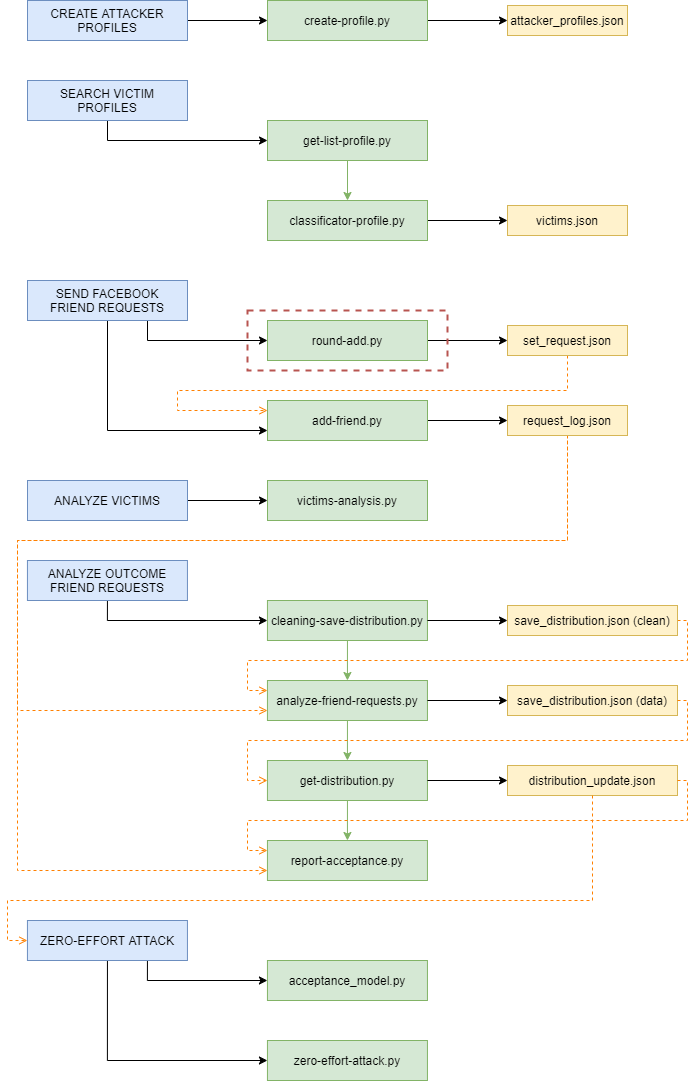
\includegraphics[width=13cm]{immagini/architecture-system.png} 
\end{center}
\label{fig:system-arc}
\end{figure}
